\documentclass[12pt]{article}
\usepackage{amsmath}
\usepackage{times}
\usepackage{anyfontsize}
\usepackage{amsfonts}
\usepackage[paperheight=12in,paperwidth=12in,margin=1in]{geometry}
\usepackage{tikz}
%\usepackage[x11names]{xcolor}
\usepackage{tcolorbox}

\usepackage{graphicx}
\graphicspath{{images/}}
\begin{document}
	
	\newtcolorbox{mybox}{colback=blue!5!white,colframe=blue}
	%\begin{tikzpicture}[remember picture,overlay]
	%\coordinate [below=12cm] (midpoint) at (current page.north);
	%\node at (current page.north west)
	%{\begin{tikzpicture}[remember picture,overlay]
	%\node[anchor=north west,inner sep=0pt,opacity=0.15] at (0,0) {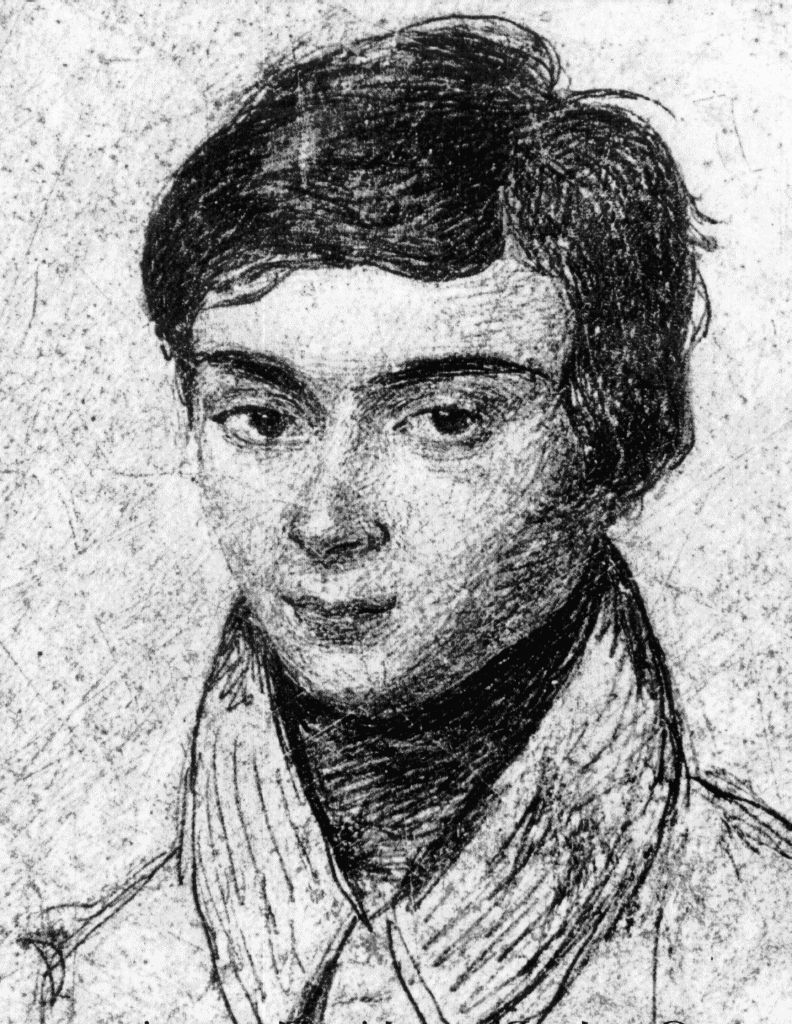
\includegraphics[width=\paperwidth]{Evariste_galois.jpg}}; \end{tikzpicture}};
	%\end{tikzpicture}
	\color{blue}
	\begin{center}
		\thispagestyle{empty}
		%\pagecolor{BrickRed}
		\color{blue}
		
		{\fontsize{40}{20}\selectfont\textbf{\underline{Sunday Special \#16}}}
		
		\vspace*{1cm}
		
		{\fontsize{35}{30}\selectfont\textbf{Send me Your Answer!}}
		\vspace*{1cm}
	\end{center}
	
	{\fontsize{30}{30}\selectfont Let $f(x)=\left(x-a_{1}\right) \ldots\left(x-a_{n}\right)+1,$ where $a_{1}, \ldots, a_{n}$ are distinct integers. Show that (i) if $n$ is odd, then $f(x)$ is irreducible over $\mathbb{Z}$ i.e. $f(x)$ cannot be factorized in the form $f(x)=p(x) q(x)$ where $p(x)$ and $q(x)$ are polynomials with integer coefficients and their degrees are less than the degree of $f(x)$ (Here the degree of $f(x)$ is $n$.) and (ii) if $n$ is even, then either $f(x)$ is irreducible over $\mathbb{Z}$ or is the square of a polynomial with integer coefficients.}
	
	\vspace{1cm}
	\begin{center}	
		{\fontsize{30}{30}\textbf{ONLY ELEMENTARY SOLUTIONS ALLOWED}}
		
		\vspace{1cm}
		
		{\fontsize{50}{60}\selectfont 
			
			$$\boldsymbol{\sum \limits_{i=0}^{Creative} Math_i = Solving}$$}
		
		%\vspace{1cm}
		
		%\begin{mybox}\Huge{\begin{center}\textbf{\textcolor{blue}{Solution $\to$}} \end{center}}\end{mybox}
	\end{center}
\end{document}

\end{document}